\subsubsection{}
\paragraph*{}
Les graphiques qui vont suivre sont tous en rapport avec une distribution
 $SBM(500,2,[0.5,0.5],a/500,b/500)$
\begin{figure}[H]
    \centering
    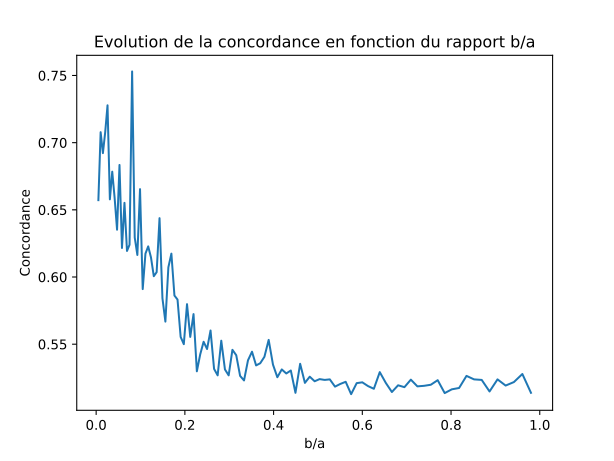
\includegraphics[width=0.5\textwidth]{figs/concordance_a_b.png}
    \caption{Evolution de la concordance en fonction du rapport $b/a$}
\end{figure}
\begin{figure}[H]
    \centering
    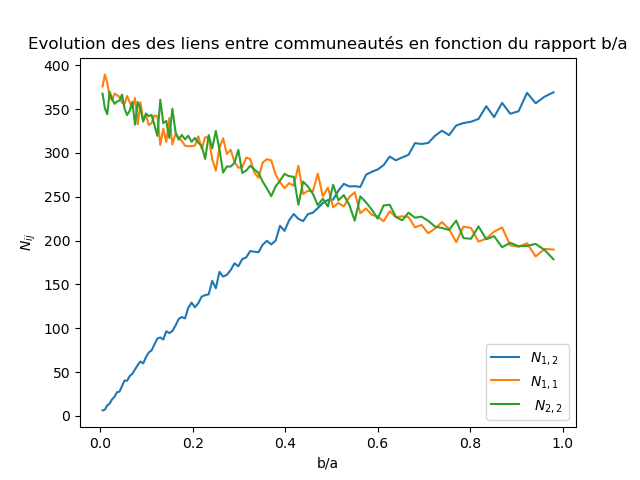
\includegraphics[width=0.5\textwidth]{figs/nij.png}
    \caption{Evolution de la concordance en fonction du rapport $b/a$}
\end{figure}

\paragraph*{}
En comparant les 2 graphiques, on remarque rapidement que moins les communeautes
ont de liens entre elles, plus l'algorithme de Metropolis-Hastings les détecte avec 
précisions. A partir d'un rapport $b/a = 0.2 $ notre algorithme ne donne aucun
résultats concluants

\subsubsection{}